% !TEX root = ../ausarbeitung.tex

\chapter{Anforderungsanalyse und Spezifikation}
\label{sec:specification}

Während der Recherche und der Konzeption des Projekts ist klar geworden, dass die zu entwickelnde Software eine relativ komplexe Architektur erfordert. Da eine Browser-basierte Webapplikation entwickelt wurde, wurde untersucht, wie die Software am besten in Teilprojekte untergliedert werden konnte. Zum einen musste das User-Interface für die Web Applikation und zum Anderen die Programmlogik entwickelt werden, welche aufgrund der benötigten Funktionalitäten (wie Datenbankanbindung und Algorithmen zur Textverarbeitung) nicht sinnvoll im Web Client implementiert werden konnte.\\
Um eine Spezifikation für die Software zu entwerfen und den zu verwendenden Software-Stack zu definieren, wurde zunächst im Gespräch mit ExpertInnen (ComputerlinguistInnen und LerntherapeutInnen) eine Anforderungsanalyse durchgeführt, die im folgendem Teil beschrieben wird. Im darauffolgenden Kapitel gehe ich Schritt für Schritt auf die Entwicklung des Gesamtsystems ein.

\section{Anforderungen an die Software}

Zunächst wurde festgestellt, welche Funktionen die Applikation den NutzerInnen bieten sollte. Dazu wurden folgende mögliche Szenarien aufgestellt:

\paragraph{Text Analyse} 
Die Nutzerin oder der Nutzer möchte einen Fließtext eingeben und von der Anwendung annotieren lassen. Nach der Eingabe soll das Ergebnis annotiert in der Applikation dargestellt werden.

\paragraph{Anpassung der annotierten Darstellung}
Die Nutzerin oder der Nutzer möchte die Einstellungen des annotierten Texts ändern. Die Texteigenschaften (Font, Zeilenabstand, Zeichenabstand) sollen angepasst werden können, sowie die Darstellung der Annotation (Farben für betonte und unbetonte Silbe, Silbenabstand, Trennzeichen zwischen Silben)

\paragraph{Export der annotierten Darstellung}
Die Nutzerin oder der Nutzer soll die Möglichkeit haben, verschiedene Formate des annotierten Texts zu exportieren, z.B. Druck, HTML oder Word.

\paragraph{Verwaltung von User Accounts}
Der Nutzerin oder dem Nutzer soll die Möglichkeit gegeben werden, ein Nutzerkonto zu erstellen um persönlich verwendete Daten (z.B. Texte oder Wortsegmentierungen) speichern zu können. Dazu sollen Funktionen und Interfaces zur Registrierung eines Nutzerkontos, Login, Logout, zum Bearbeiten der Nutzerinformationen und zum Löschen des Accounts bereitgestellt werden.

\paragraph{Behandlung unbekannter Wörter}
Die Nutzerin oder der Nutzer kann nacheinander die Segmentierung von Wörtern, die durch das System nicht eindeutig bestimmt werden konnten, selbst manuell festlegen.

\paragraph{Bestimmung der Segmentierung unbekannter Wörter}
Für ein unbekanntes Wort wählt die Nutzerin oder der Nutzer in einem neuen View die Segmentierung selbst aus. Dafür sollen folgende Möglichkeiten gegeben werden:
\begin{itemize}
	\item Input aus G2P Systemen wie MARY TTS
	\item Manuelle Segmentierung mit geeignetem User Interface
	\item Eventuell weitere Quellen für die Segmentierung (z.B. Duden oder Wictionary)
\end{itemize}

\paragraph{Speicherung von Nutzer Segmentierungen}
Von der Nutzerin oder dem Nutzer hinzugefügte Segmentierungen sollen (lokal für das Nutzerkonto) gespeichert werden können und beim nächsten Vorkommen in einem Text automatisch verwendet werden.

\paragraph{Speicherung und Wiederverwendung von Annotationskonfigurationen für Texte}
Die Einstellungen, die eine Nutzerin oder ein Nutzer an einem annotierten Text vorgenommen hat, sollen als Vorlage für andere Texte gespeichert werden können. In den Annotationseinstellungen eines Textes soll eine zuvor gespeicherte Konfiguration wiederverwendet werden können.

\paragraph{Speicherung und Wiederverwendung von Nutzertexten}
Analysierte Texte sollen von der Nutzerin oder dem Nutzer zusammen mit der verwendeten Konfiguration gespeichert werden können. Den Texten werden Metadaten zugeordnet, z.B. Titel, Thema, Niveau oder Zielgruppe. Im Nutzerbereich werden die Texte, die NutzerInnen hinzugefügt haben, geeignet strukturiert dargestellt. Es soll die Möglichkeit gegeben werden, den gespeicherten Text erneut analysieren zu lassen.

\paragraph{Verifizierung unbekannter Wörter}
Manuelle Segmentierungen von unbekannten Wörtern müssen auf Korrektheit überprüft werden können. Dazu sollen alle NutzerInnen aufgefordert werden, die Einträge, die mit anderen Nutzerkonten erstellt wurden, zu überprüfen. In einem Fenster, ähnlich zur manuellen Segmentierung, sollen die NutzerInnen fremde Einträge bestätigen oder Gegenvorschläge übermitteln können.

\paragraph{Expertennutzer}
ExpertInnen (z.B. LinguistInnen oder LerntherapeutInnen) sollen sich als Solche bei der Erstellung eines Accounts identifizieren können. Bei der Wort-Verifizierung zählt die Stimme der ExpertennutzerInnen mehr als die von NutzerInnen, die keine Experten sind.

Hieraus lassen sich folgende grundlegende Anforderungen an die Software spezifizieren:

\begin{itemize}
	\item Service zur Textanalyse
	\item Datenbank für Wörter und deren Segmentierung
	\item Service zur Manipulation der Wortdatenbank
	\item Speicherung nutzerspezifischer Daten
	\item Service zur Nutzerverwaltung
	\item Geeignetes User Interface zur Darstellung von Texten, Verwaltung der Nutzerdaten und zur Interaktion mit dem System
\end{itemize}

\subsection{User Interface}
Im nächsten Schritt wurde, von den Szenarien und Anforderungen ausgehend, das Design für ein geeignetes User Interface erarbeitet. Tabelle \ref{table:navigation} zeigt die für die Navigation wichtigsten Komponenten.

\begin{table}[h!]
	\centering
	\begin{tabular}{|l|p{8cm}|}
		\hline
		Hauptnavigationskomponente & Unterpunkte / Funktionen \\
		\hline
		\hline
		Begrüßungsseite (Home) & Informationen zum Hintergrund der Applikation und zu verfügbaren Funktionen\\
		\hline
		Textanalyse & Eingabe und Analyse von Texten, Annotation und Darstellung des Textes, sowie Funktionen zum Druck und Export\\
		\hline
		Nutzerkonto & Login, Registrierung, Verwaltung des Nutzerkontos und nutzerspezifischer Daten \\
		\hline
		Verifizierung & Verifizierung manuell segmentierter Wörter \\
		\hline
	\end{tabular}
	\caption{Hauptkomponenten der Navigationsstruktur}
	\label{table:navigation}
\end{table}

\subsubsection{Informationsstruktur}

Mithilfe dieser Überlegungen wurde festgelegt, dass es eine horizontale Navigationsleiste mit den vier aufgelisteten Hauptnavigationskomponenten geben soll. Der Link zum Nutzerkonto sollte aufgrund von Nutzergewohnheiten gesondert, rechtsbündig in der Navigationsleiste platziert werden (Abbildung \ref{fig:navigation}). Jeder Punkt der Navigation soll Einstiegspunkt in eine Hauptkomponente der Applikation sein, es gibt keine weiteren Ebenen in der Navigationshierarchie, da die Anzahl der Komponenten überschaubar ist. Daher wird auch auf andere Navigationsmöglichkeiten, wie z.B. eine seitenweite Suche verzichtet.


\begin{figure}[h!]
	\centering
	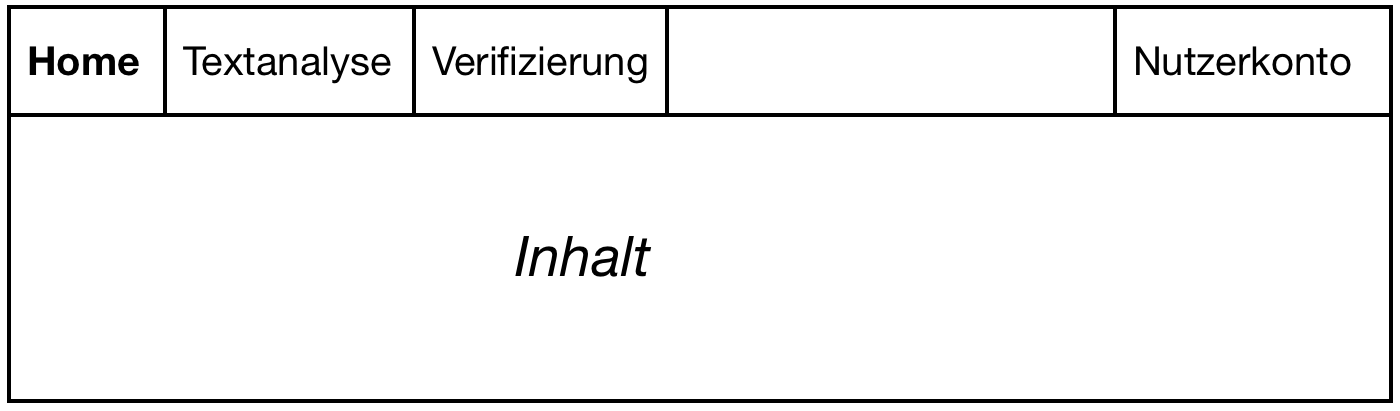
\includegraphics[width=.8\linewidth]{figures/navigation}
	\caption{Navigationsstruktur}
	\label{fig:navigation}
\end{figure}

\subsubsection{Farbschema}

Als Nächstes wurde ein möglichst ansprechendes Farbschema gesucht. Hierfür wurde mit einem Farbrad (es wurde Adobe Color CC verwendet, \textit{https://color.adobe.com}) zwei Komplementärfarben als Hauptfarben ausgesucht (s. Abbildung \ref{fig:colors}). Die blaue Farbe wurde vor allem für Links eingesetzt, eine hellere Version für Links im Hover Zustand. Eine weitere, ins Türkis gehende Abstufung wurde für Rahmen beim Gruppieren von Elementen auf der Seite verwendet. Der beige Farbton kommt als Hintergrundfarbe für die Navigationsleiste zum Einsatz.

\begin{figure}[h!]
	\centering
	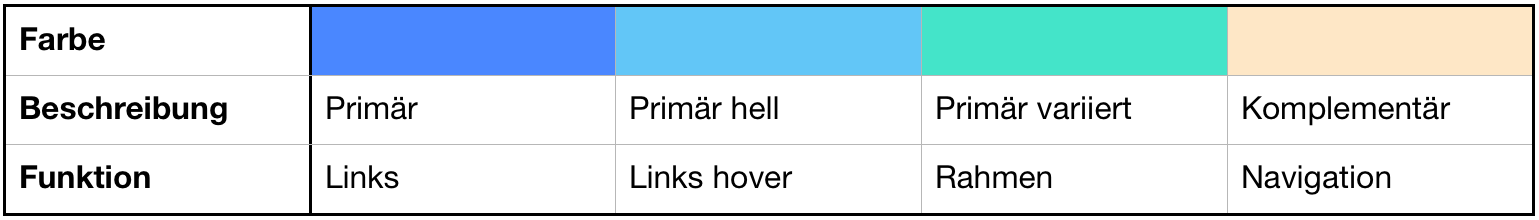
\includegraphics[width=.95\linewidth]{figures/farbschema}
	\caption{Farbschema aus Komplementärfarben}
	\label{fig:colors}
\end{figure}


\section{Softwarestack}

Bei der Vielseitigkeit der verschiedenen Anforderungen ist die Wahl der zu verwendenden Technologien nicht unerheblich. Programmiersprachen und Frameworks mussten sorgfältig ausgewählt werden, um für jedes Teilproblem eine passende Lösung zu entwickeln.\\
Die erste wichtige Unterteilung fand zum Einen in ein Frontend statt, welches die Schnittstelle den NutzerInnen darstellt und zum Anderen in ein Backend, das die vom System verwendeten Daten speichert, manipuliert und diese nach Aufbereitung mit entsprechenden Algorithmen an das Frontend schickt (s. Abbildung \ref{fig:frontendbackend}). Eine genaue Beschreibung über den Aufbau und die Funktion von Front- und Backend wird in Kapitel 4 gegeben.\\

\begin{figure}[h!]
	\centering
	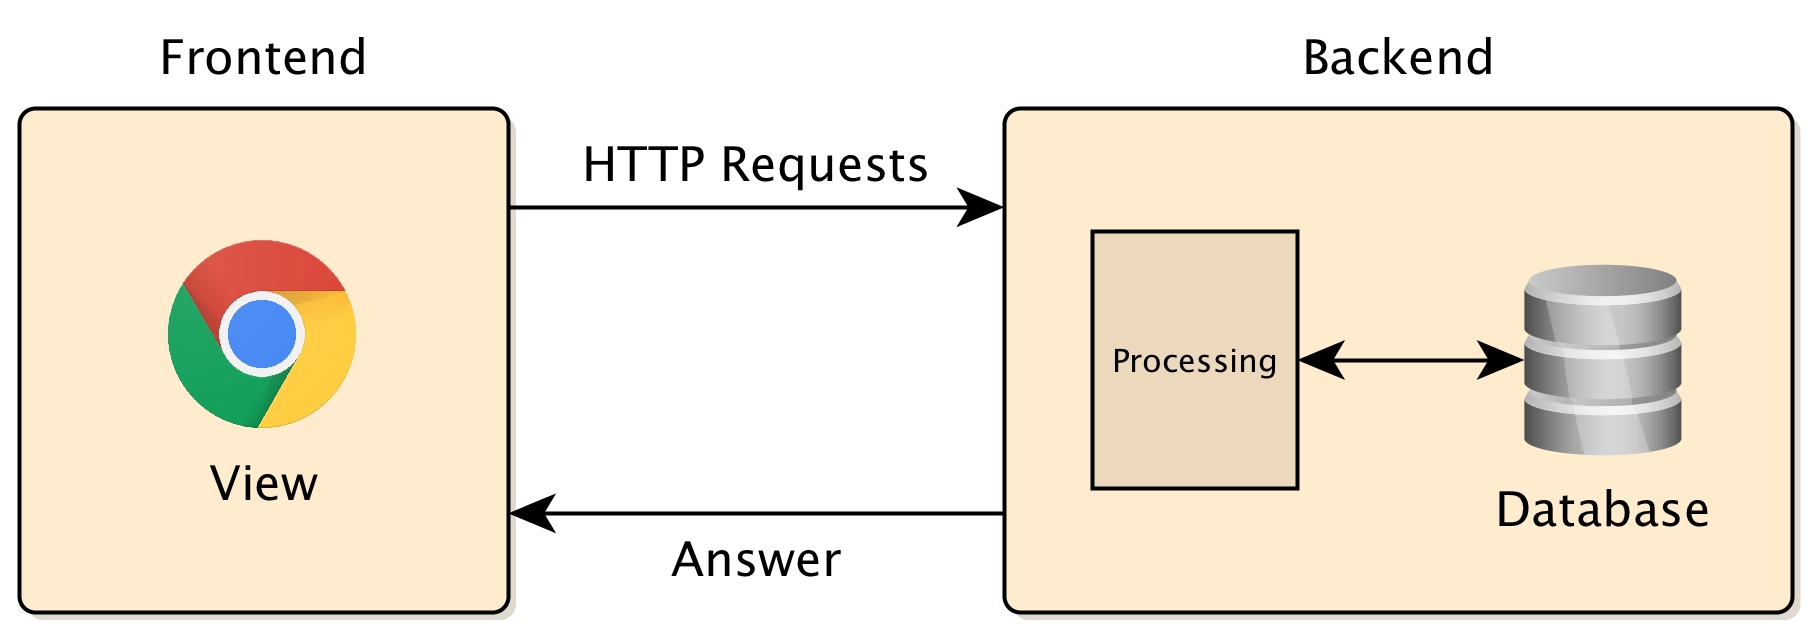
\includegraphics[width=.8\linewidth]{figures/frontendbackend}
	\caption{Kommunikation zwischen Front- und Backend}
	\label{fig:frontendbackend}
\end{figure}

Diese Aufteilung ist in der Webentwicklung weit verbreitet\cite{Fielding:2000:ASD:932295} und bietet einige Vorteile gegenüber einem komplett integriertem Gesamtsystem:

\begin{itemize}
	\item Klare Trennung von Darstellung und Datenverarbeitung
	\item Einfachere Fehlersuche durch kleinere Komponenten
	\item Bei der Entwickelung zusätzlicher Frontends (z.B. für Android oder iOS) muss nur ein neuer Teil des Softwaresystems entwickelt werden, während das Backend gleich bleibt.
	\item Arbeitsaufteilung im Entwicklerteam (relevant bei Weiterentwicklung der Applikation mit mehreren Personen)
\end{itemize}

\subsection{Verwendete Technologien}
Bei den verschiedenen zu realisierenden Zielen gibt es für jedes Teilziel Technologien, die Vorteile gegenüber Anderen bieten. Die Verwaltung von Datenbanken ist zum Beispiel besser mit einer server-seitigen Skriptsprache zu implementieren, als mit den Möglichkeiten, die das Frontend bietet. Im Web Frontend dagegen sind gewisse Technologien wie \textit{HTML}, \textit{CSS} und \textit{JavaScript} Standard, die zwangsläufig verwendet werden müssen. Daher wird in der Applikation eine Vielzahl verschiedener Technologien verwendet, eine Übersicht ist hier gegeben:

\begin{itemize}
	\item Backend: \textit{Python} mit den Frameworks \textit{Flask}, \textit{Spacy} und \textit{Sqlalchemy}
	\item Frontend: \textit{HTML}, \textit{CSS}, \textit{JavaScript} und \textit{AngularDart}
	\item Kommunikation zwischen Front- und Backend im \textit{JSON} Format
	\item Deployment mit \textit{Apache} auf einem \textit{AWS} Server
\end{itemize}

Im Folgenden werden die einzelnen Technologien und die Gründe für deren Verwendung beschrieben.

\subsection{Backend}
\label{sec:backend}

Um die Entwicklung des Backends möglichst einfach zu halten, wurde zunächst untersucht, ob ein fertiges Backend (Backend-a- a-Service) verwendet werden kann. Hierfür kämen z.B. fertige Services wie MongoDB oder Firebase mit integrierter NoSQL Datenbank infrage\cite{almootassem2017}.\\
Zunächst wurde Firebase genauer untersucht und in Verbindung mit dem Frontend getestet. Prinzipiell war es gut möglich eine Verbindung mit dem Frontend herzustellen (Daten in der Firebase Datenbank können mit HTTP Requests geschrieben und gelesen werden). Die Möglichkeiten des Backends beschränkten sich allerdings auf Datenmanipulation und Cloud Code (server-seitiges JavaScript in Firebase).\\
Ein Problem dabei war, dass komplexere Logik wie das \textit{Natural Language Processing} nur entweder im Frontend oder im Backend mit \textit{JavaScript} implementiert werden konnte. NLP Frameworks, wie es sie z.B. in \textit{Python} oder \textit{Java} gibt, konnten somit nicht verwendet werden. Wurde der Text im Frontend in einzelne Wörter zerlegt und diese in der Firebase Datenbank nachgeschlagen, musste zudem für jedes Wort ein eigener HTTP Request geschickt werden, was zu unbefriedigenden Antwortzeiten führte.\\

Aufgrund der beschriebenen Probleme wurde parallel ein alternatives Backend in \textit{Python} implementiert. Die Entwicklung der Softwarearchitektur wurde an den \textit{Representational State Transfer} (REST) angelehnt. Dieser beschreibt Prinzipien und Restriktionen für die Konzeption von Webarchitekturen\cite{Fielding:2000:ASD:932295}. Diese Lösung brachte zwar wiederum eigene Schwierigkeiten und Probleme mit sich (s. Abschnitt \ref{sec:deployment}), wurde aber für die kurzfristig bessere und schneller zu entwickelnde Variante erachtet und daher weiter verfolgt. Da in der Praxis die Entwicklung und Wartung eines eigenen Backends einen erheblichen Mehraufwand bedeuten kann, wäre weiterführend auch eine kombinierte Lösung denkbar. Hierfür könnt ein Backend-as-a-Service wie Firebase benutzt, aber zwischen Front- und Backend noch eine weitere Schicht eingesetzt werden, welche Programmlogik enthält und NLP Berechnungen durchführen kann.

Die Einhaltung der REST Restriktionen (z.B. muss das Backend zustandslos sein und die Anfragen müssen resourcenorientiert formuliert werden) wurden so gut es im Rahmen der Arbeit möglich war eingehalten. Allerdings konnte die Konzeption einer konsequenten Softwarearchitektur nicht im Vordergrund stehen, da die entwickelte Applikation lediglich als Prototyp betrachtet werden muss. Im Folgenden werden die Technologien, die für das Python Backend benutzt wurden vorgestellt.

\paragraph{Python}
\label{sec:python}

Die Verwendung von \textit{Python}\cite{vanRossum2011} im Backend brachte einige Vorteile für die Effizienz der Applikation, sowie für eine gute Strukturierung des Projekts, da ein großer Teil der Programmlogik im Backend abgebildet und somit die Komplexität des Frontends entlastet werden konnte. Zudem konnten nützliche Frameworks für NLP oder für die Verarbeitung der HTTP Requests benutzt werden.

\paragraph{Flask}
\label{sec:flask}

ist ein \textit{Python} Framework für die Webentwicklung. Es kann z.B. eingesetzt werden, um Webseiten an Clients auszuliefern, allerdings auch um eine API zu entwickeln, welche nur Daten an einen Client schickt anstatt ganzer Webseiten\cite{Grinberg:2014:FWD:2621997}. Bei der Entwicklung einer Flask Applikation wird zunächst im Python Skript ein Applikationsobjekt angelegt. Die Applikation kann in Python konfiguriert und mit einem Funktionsaufruf gestartet werden.\\
Alle beim Server ankommenden HTTP Requests werden von \textit{Flask} automatisch verarbeitet. Das Verhalten für eigene Routen kann durch annotierte Funktionsdefinitionen angepasst werden. Abbildung \ref{fig:flask} zeigt ein Beispiel, wie das Erstellen einer Ressource mit einem HTTP Request an eine selbst definierte Methode weitergeleitet wird. Zudem kann im \texttt{methods} Array definiert werden für welche HTTP Methoden die Route gilt.\\
In den zu den Routen definierten Methoden können Backend Services (s. Abschnitt \ref{sec:etwicklung-backend}) aufgerufen werden, welche die Daten der Applikation abfragen und entsprechend aufbereitet zurückgeben. 

\begin{figure}
	\begin{lstlisting}
@app.route('/user/word/add', methods=['POST'])
def user_add_word():
...
	\end{lstlisting}
	\caption{Definition von \textit{Flask} Routen}
	\label{fig:flask}
\end{figure}

\paragraph{Spacy}
\label{sec:spacy}

Für die Erledigung der linguistischen Aufgaben in der Applikation wurde nach einem effektiven NLP Parser gesucht. Hierfür wurde erst das \textit{Natural Language Toolkit} (NLTK)\cite{Bird2004a} ausprobiert. Hierbei handelt es sich um eine Reihe von Python Modulen für die Durchführung von NLP Aufgaben. Es wurde Open Source und vor allem für akademische Zwecke entwickelt und wurde für die Verwendung in der Applikation als geeignet befunden.\\
Zusätzlich wurde der \textit{Spacy} Parser untersucht, ein weiteres Python NLP Framework. Bei der Erstellung von \textit{Spacy} wurde unter anderem der Fokus auf Performanz gelegt, entwickelt wurde es in \textit{Cython} (eine zu Python kompatible Sprache, welche aber bei der Kompilierung nach C übersetzt wird), was zu schnellerer Ausführung im Vergleich zum Python Interpreter führt.\\
Eigenes Testen und andere Quellen haben gezeigt, dass der \textit{Spacy} Parser aufgrund seiner Effizienz\cite{Stent2015} und Benutzbarkeit für die Aufgabe sehr gut geeignet ist. Er wurde daher in der Applikation zum Parsen des Eingabetexts, als Tokenizer und zur Bestimmung der Part-of-Speech Tags anstelle von NLTK benutzt.

\subsection{Frontend}

Für die Entwicklung einer Webapplikation sind viele Technologien schon vorgegeben. Der Einsatz von \textit{HTML}, \textit{CSS} und \textit{JavaScript} auf der Client Seite ist zur Darstellung der Applikation im Browser notwendig und praktisch unverzichtbar. Im Gegensatz zu einer normalen Website wurde hier eine Single-View-Application entwickelt, d.h. anstatt bei Nutzerinteraktionen eine neue HTML Datei zu laden, verändert die Applikation den Inhalt der Seite (das Document Object Model, DOM) dynamisch mit Skripten\cite{mikowski2013single}.\\

JavaScript könnte als einzige Frontend Sprache verwendet werden. Das Modell der Applikation würde dann mit verschiedenen Skripten abgebildet werden und die Kommunikation mit dem Backend würde über AJAX Anfragen erfolgen. Da JavaScript aber über keine starke Typisierung verfügt und eine Strukturierung der Anwendung durch Klassen nur bedingt möglich ist, wurden Alternativen für die Frontendsprache gesucht. Eine Möglichkeit hier ist die Generierung von JavaScript aus anderen Sprachen. Hierbei wird Code in einer anderen Hochsprache geschrieben und für die Ausführung im Browser mit einem Compiler nach JavaScript übersetzt. Dieser Ansatz wird von einigen Sprachen oder Frameworks unterstützt, z.B. CoffeeScript, TypeScript, GWT (Java) oder AngularDart. Nach dem Erwerb eines Überblicks über diese Technologien entschied ich mich dafür, die von Google entwickelte Sprache \textit{Dart} und das \textit{AngularDart} Framework zu verwenden, deren Funktionsweise im folgenden Abschnitt näher erklärt wird.

\subsubsection{AngularDart}
\label{sec:angulardart}

Dart ist eine von Google entwickelte Programmiersprache, die z.B. in einigen Google Tools (z.B. AdWords oder interne Tools für Marketing und Sales) verwendet wird. Sie wird nicht in erster Linie für die Webentwicklung benutzt, sondern kann durch entsprechende Kompilierung z.B. auch für die Backend Entwicklung oder für iOS und Android Applikationen verwendet werden.\\
Für die Erstellung einer Webanwendung mit Dart wird das Framework \textit{AngularDart}\cite{angularDart}  benutzt. Dieses wurde nach dem Vorbild der Technologien \textit{AngularJS} und \textit{Angular} entwickelt, wobei Ersteres mit reinem JavaScript programmiert wird und bei \textit{Angular} die Programmiersprache \textit{TypeScript} zum Einsatz kommt. Bei \textit{AngularDart} wird der in \textit{Dart} erstellte Code beim Build mit dem \textit{dart2js} Compiler nach \textit{JavaScript} übersetzt.

\begin{figure}[h!]
	\centering
	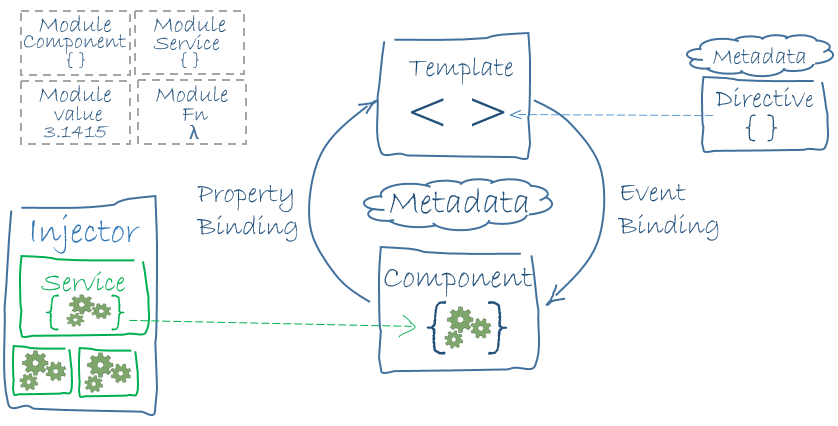
\includegraphics[width=.8\linewidth]{figures/angulardart}
	\caption{Funktionsweise einer AngularDart Webanwendung\cite{angularDart}}
	\label{fig:angulardart}
\end{figure}

Abbildung \ref{fig:angulardart} gibt einen Überblick über die Funktionsweise einer AngularDart Webanwendung. Bei dieser Architektur wird die Programmlogik in \textit{Services} abgebildet welche durch \textit{Dependency Injection} in anderen Programmteilen verwendet werden können. Das Layout der Website wird von den eingebundenen \textit{Komponenten} bestimmt. Eine AngularDart Komponente besteht aus einem HTML \textit{Template} und einer (Dart) Komponentenklasse und kann in jedem anderen HTML Template eingebunden werden. Es gibt sowohl von AngularDart vordefinierte Komponenten als auch die Möglichkeit, eigene Komponenten zu entwickeln.\\
Das Template verwendet einen eigenen Syntax bei dem Angular \textit{Direktiven} in HTML aufgerufen werden können. Der Template Syntax bietet z.B. die Möglichkeiten mit \textit{Property Binding} auf Daten der Komponentenklasse zuzugreifen, oder mit den Direktiven \textit{ngIf} oder \textit{ngFor} Daten bedingt darzustellen.\\Werden in der Komponentenklasse Daten verändert, wird dies automatisch von AngularDart detektiert. Infolgedessen wird durch das \textit{Property Binding} die Anzeige in der HTML Seite automatisch angepasst. Eine genaue Beschreibung der Funktionsweise liefert die AngularDart Dokumentation\cite{angularDart}.

\subsection{Deployment}
\label{sec:deployment}

Der Output der AngularDart Applikation ist eine Website aus HTML und JavaScript. Um diese verfügbar zu machen, muss sie auf einem Webserver gehostet werden, der mittels Namensauflösung über DNS mit einer URI erreichbar ist. Hier wurde für den Prototyp der Applikation über die Amazon Web Services (AWS) ein kostenloser Zugang angelegt, mit dem eine virtuelle Maschine (VM) erstellt werden konnte (EC2 Service\cite{amazonec2}), die man z.B. über SSH erreichen kann. Sowohl die AngularDart Applikation, als auch das Python Backend wurden auf die VM übertragen, jedoch auf verschiedenen Ports gestartet, das Frontend mit Apache2 auf Port 8001, das Backend mit Python3 auf Port 8000. Alle im Frontend ausgehenden Anfragen rufen das Backend über die Server URI des Amazon Servers auf Port 8000 auf.

\begin{table}[h!]
	\centering
	\begin{tabular}{|l|l|l|}
		\hline
		\textbf{Adresse} & \textbf{Port} & \textbf{Applikation}\\
		\hline
		\hline
		http://ec2-\textit{<...>}.compute.amazonaws.com:8001 & 8001 & Frontend, mit Apache2 gehostet\\
		\hline
		http://ec2-\textit{<...>}.compute.amazonaws.com:8000 & 8000 & Python3 Flask Backend\\
		\hline
	\end{tabular}
	\caption{Die URIs beginnen mit \textit{\qq{ec2}} und enden mit der Adresse von Amazon AWS. Front- und Backend wurden mit unterschiedlichen Ports auf dem gleichen Server gehostet.}
\end{table}

Der beschriebene Weg wurde gewählt um die Webapplikation schnell und einfach verfügbar zu machen. Netzwerksicherheit wurde im Rahmen der Arbeit vernachlässigt, da der Schwerpunkt auf der Entwicklung der User Interfaces und auf den NLP Aufgaben lag. So wird z.B. nur das HTTP Protokoll verwendet, nicht \textit{HTTPS}. Die Verwendung von zwei verschiedenen Ports für die Anwendung führt zu Problemen, wenn man Sicherheitskonzepte wie die HTTP Authentifizierung umsetzen will. Die meisten Webbrowser implementieren die \textit{Same Origin Policy} und beschränken die Kommunikation zwischen verschiedenen Quellen (\textit{Cross-Origin Resource Sharing}\cite{kesteren2010}). Als Behilfslösung wurden für die Authentifizierung Mailadresse und Passwort als Form Data von HTTP POST Requests mit übertragen. Dies führte auch dazu, dass in allen Anfragen, bei denen die Authentifizierung übermittelt werden musste, die POST Methode benutzt wurde (s. Tabelle \ref{table:backendroutes}) und nicht die für die REST Architektur üblichen Methoden wie \textit{PUT} oder \textit{DELETE} eingesetzt werden konnten.\\
Bei einer Weiterentwicklung der Applikation wäre hier denkbar, z.B. entweder auch das mit AngularDart erstellte Frontend als Teil der \textit{Flask} Applikation zu hosten (und somit beides von einer Quelle aus und auf einem Port auszuliefern), oder ein Backend-as-a-Service wie Firebase (s. Abschnitt \ref{sec:backend}) für die sicherheitskritischen Ressourcen zu verwenden, da diese Backends von Haus aus Authentifizierung anbieten.